\documentclass[landscape,fontscale=0.292,archE]{baposter}
% a0paper,
\usepackage[vlined]{algorithm2e}
\usepackage{times}
\usepackage{calc}
\usepackage{url}
\usepackage{graphicx}
\usepackage{amsmath,amsthm,amssymb}
\newtheorem{theorem}{Theorem}
\newtheorem{corollary}{Corollary}
\usepackage{relsize}
\usepackage{multirow}
\usepackage{booktabs}

\usepackage{graphicx}
\usepackage{multicol}
\usepackage[T1]{fontenc}
\usepackage{ae}
\usepackage{enumitem}

\usepackage{colortbl}
\usepackage{xcolor}
\graphicspath{{images/}}
\usepackage{color}

\setlist[itemize]{leftmargin=*,nosep}
 \setlength{\columnsep}{0.7em}
 \setlength{\columnseprule}{0mm}

\usepackage{subcaption}
% %%%%%%%%%%%%%%%%%%%%%%%%%%%%%%%%%%%%%%%%%%%%%%%%%%%%%%%%%%%%%%%%%%%%%%%%%%%%%%%%
% % Save space in lists. Use this after the opening of the list
% %%%%%%%%%%%%%%%%%%%%%%%%%%%%%%%%%%%%%%%%%%%%%%%%%%%%%%%%%%%%%%%%%%%%%%%%%%%%%%%%
 \newcommand{\compresslist}{%
 \setlength{\itemsep}{0pt}%
 \setlength{\parskip}{0pt}%
 \setlength{\parsep}{0pt}%
 }
\renewcommand{\rmdefault}{ptm} % Arial
\renewcommand{\sfdefault}{ptm} % Arial

%%%%%%%%%%%%%%%%%%%%%%%%%%%%%%%%%%%%%%%%%%%%%%%%%%%%%%%%%%%%%%%%%%%%%%%%%%%%%
%% Begin of Document
%%%%%%%%%%%%%%%%%%%%%%%%%%%%%%%%%%%%%%%%%%%%%%%%%%%%%%%%%%%%%%%%%%%%%%%%%%%%%
\begin{document}
%%%%%%%%%%%%%%%%%%%%%%%%%%%%%%%%%%%%%%%%%%%%%%%%%%%%%%%%%%%%%%%%%%%%%%%%%%%%%
%% Here starts the poster
%%---------------------------------------------------------------------------
%% Format it to your taste with the options
%%%%%%%%%%%%%%%%%%%%%%%%%%%%%%%%%%%%%%%%%%%%%%%%%%%%%%%%%%%%%%%%%%%%%%%%%%%%%
\begin{poster}{
 % Show grid to help with alignment
 grid=false,
 columns=5,
 % Column spacing
 colspacing=0.7em,
 % Color style
 headerColorOne=cyan!20!white!90!black,
 borderColor=cyan!30!white!90!black,
 % Format of textbox
 textborder=faded,
 % Format of text header
 headerborder=open,
 headershape=roundedright,
 headershade=plain,
 background=none,
 bgColorOne=cyan!10!white,
 headerheight=0.12\textheight}
 % Eye Catcher
 {
      
\includegraphics[width=0.08\linewidth]{PolyU_logo.png}
      \makebox[0.01\textwidth]{} 
      %\raisebox{0.08\height}{
\includegraphics[width=0.10\linewidth]{CUHK_logo.jpg}}
      %\makebox[0.04\textwidth]{} 
 }
 % Title
 {\sc\Huge\bf A Trilateral Weighted Sparse Coding Scheme \\ for Real-World Image Denoising}
 % Authors
 {
 \vspace{0.1em} 
 \normalsize{Jun Xu$^1$, Lei Zhang$^1$, David Zhang$^{1,2}$ }
 \\[0.1em]
 {\small
 $^1$ Department of Computing, Hong Kong Polytechnic University, Hong Kong SAR, China
 \\
 $^2$ School of Science and Engineering, The Chinese University of Hong Kong (Shenzhen), Shenzhen, China
 \\[0.1em] 
 }
 }
 % University logo
 {
    \begin{tabular}{r}
        \includegraphics[width=0.15\linewidth]{cropped-Logo_ECCV18_RGB_1200x280}
    \end{tabular}
 }
%%%%%%%%%%%%%%%%%%%%%%%%%%%%%%%%%%%%%%%%%%%%%%%%%%%%%%%%%%%%%%%%%%%%%%%%%%%%%%
%%% Now define the boxes that make up the poster
%%%---------------------------------------------------------------------------
%%% Each box has a name and can be placed absolutely or relatively.
%%% The only inconvenience is that you can only specify a relative position 
%%% towards an already declared box. So if you have a box attached to the 
%%% bottom, one to the top and a third one which should be inbetween, you 
%%% have to specify the top and bottom boxes before you specify the middle 
%%% box.
%%%%%%%%%%%%%%%%%%%%%%%%%%%%%%%%%%%%%%%%%%%%%%%%%%%%%%%%%%%%%%%%%%%%%%%%%%%%%%

%%%%%%%%%%%%%%%%%%%%%%%%%%%%%%%%%%%%%%%%%%%%%%%%%%%%%%%%%%%%%%%%%%%%%%%%%%%%%%
    \vspace{-2mm}
\headerbox{\bf\color{blue} Problem, Motivation, and Contributions}{name=contribution,column=0,row=0,span=2}{
    \textbf{\color{blue}Goal:} Estimating the latent clean image from the input real-world noisy image.
    
    \textbf{\color{blue}Motivation:} Realistic noise show channel-wise and locally signal dependent property.
    \begin{center}
        \vspace{-2mm}
        \centering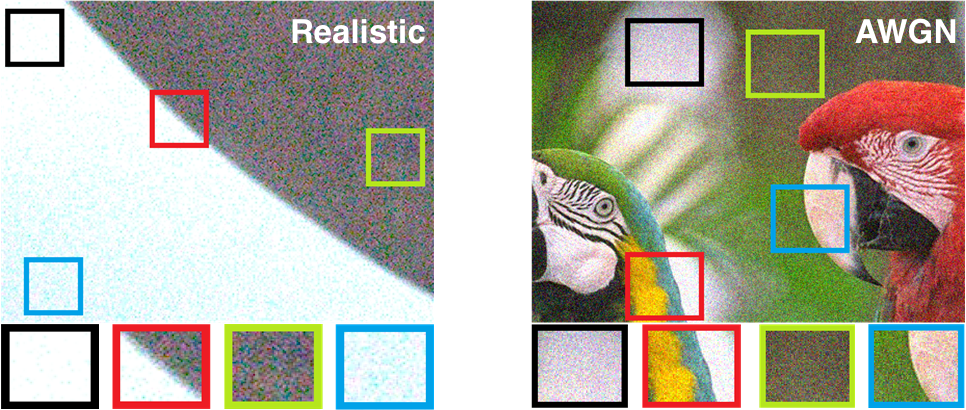
\includegraphics[width=0.95\linewidth]{images/compare}
        \centering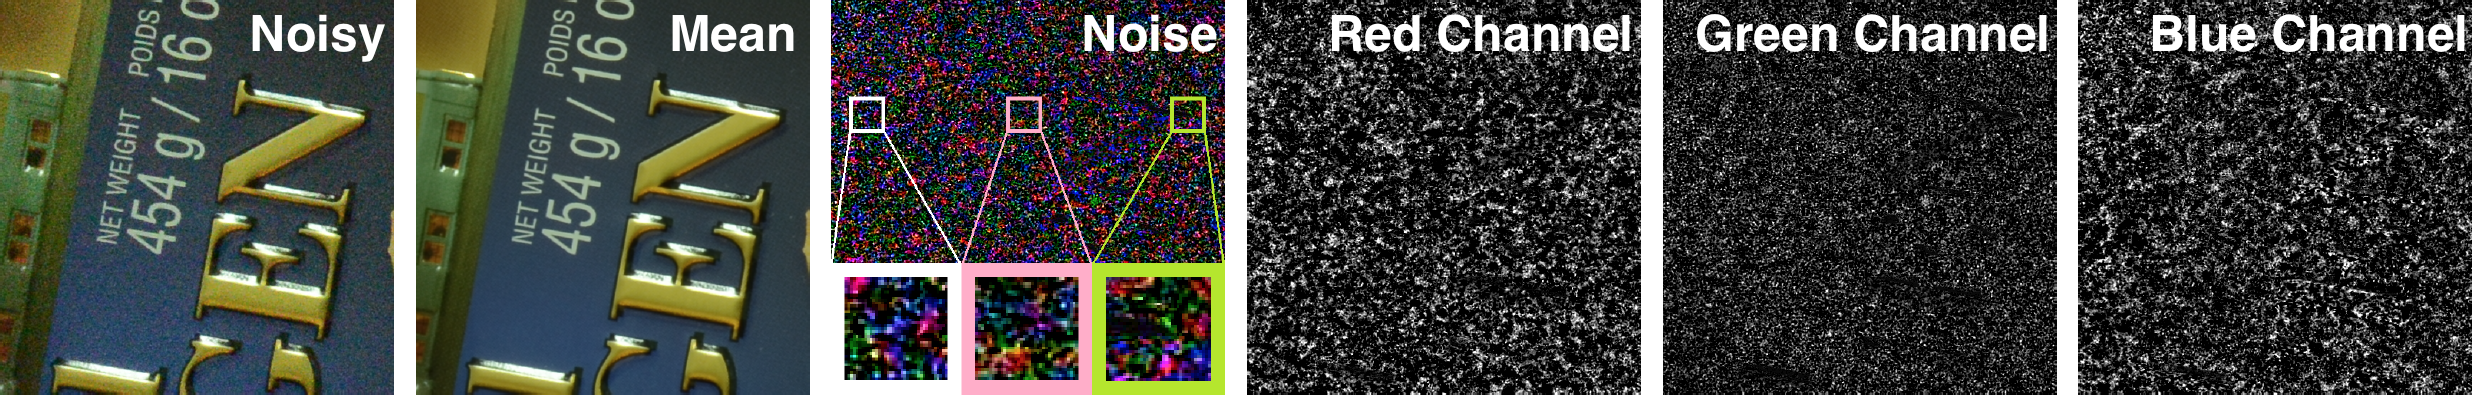
\includegraphics[width=0.95\linewidth]{images/channelwise}
    \end{center}
    \vspace{-1mm}
    
    \textbf{\color{blue}Contributions:}
    \begin{itemize}
        \item Propose a trilateral weighted sparse coding (TWSC) scheme for real-world denoising;
        \item TWSC achieves much better performance than state-of-the-art denoising methods.
    \end{itemize}    
        \vspace{-1mm}
}

%%%%%%%%%%%%%%%%%%%%%%%%%%%%%%%%%%%%%%%%%%%%%%%%%%%%%%%%%%%%%%%%%%%%%%%%%%%%%%
\headerbox{\bf\color{blue} Theoretical Analysis}{name=analysis,column=2,row=0,span=3}{
    \begin{minipage}[t]{0.4\textwidth}
        \textbf{\color{blue}Convergence:} 
        \vspace{-2mm}
        \begin{center}
            \includegraphics[width=0.8\textwidth]{images/Convergence.png}
        \end{center}
    \end{minipage}
    \begin{minipage}[t]{0.6\textwidth}
        \textbf{\color{blue}Existence of the \textcolor{red}{Solution} to ADMM (a):} 
        \vspace{-4mm}
        \begin{center}
           \begin{theorem}
\label{th1}
Assume that $\mathbf{A}\in\mathbb{R}^{3p^2\times 3p^2}$, $\mathbf{B}\in\mathbb{R}^{M\times M}$ are both symmetric and positive semi-definite matrices.\ If at least one of $\mathbf{A}, \mathbf{B}$ is positive definite, the Sylvester equation $\mathbf{A}\mathbf{C}
+
\mathbf{C}\mathbf{B}
=
\mathbf{E}$ has a unique solution for $\mathbf{C}\in \mathbb{R}^{3p^2\times M}$.
\end{theorem}

\begin{corollary}
The  \textcolor{red}{Solution} to ADMM (a) exists and is unique.
\end{corollary}
        \end{center}
    \end{minipage}
}    
    
%%%%%%%%%%%%%%%%%%%%%%%%%%%%%%%%%%%%%%%%%%%%%%%%%%%%%%%%%%%%%%%%%%%%%%%%%%%%%%
\headerbox{\bf\color{blue} Experimental Results}{name=results,column=2,below=analysis,span=3}{
    \begin{minipage}[t]{0.5\textwidth}
        \textbf{\color{blue}Quantitative Comparisons on AWGN Removal:}
        \vspace{-2mm}
        \begin{center}
            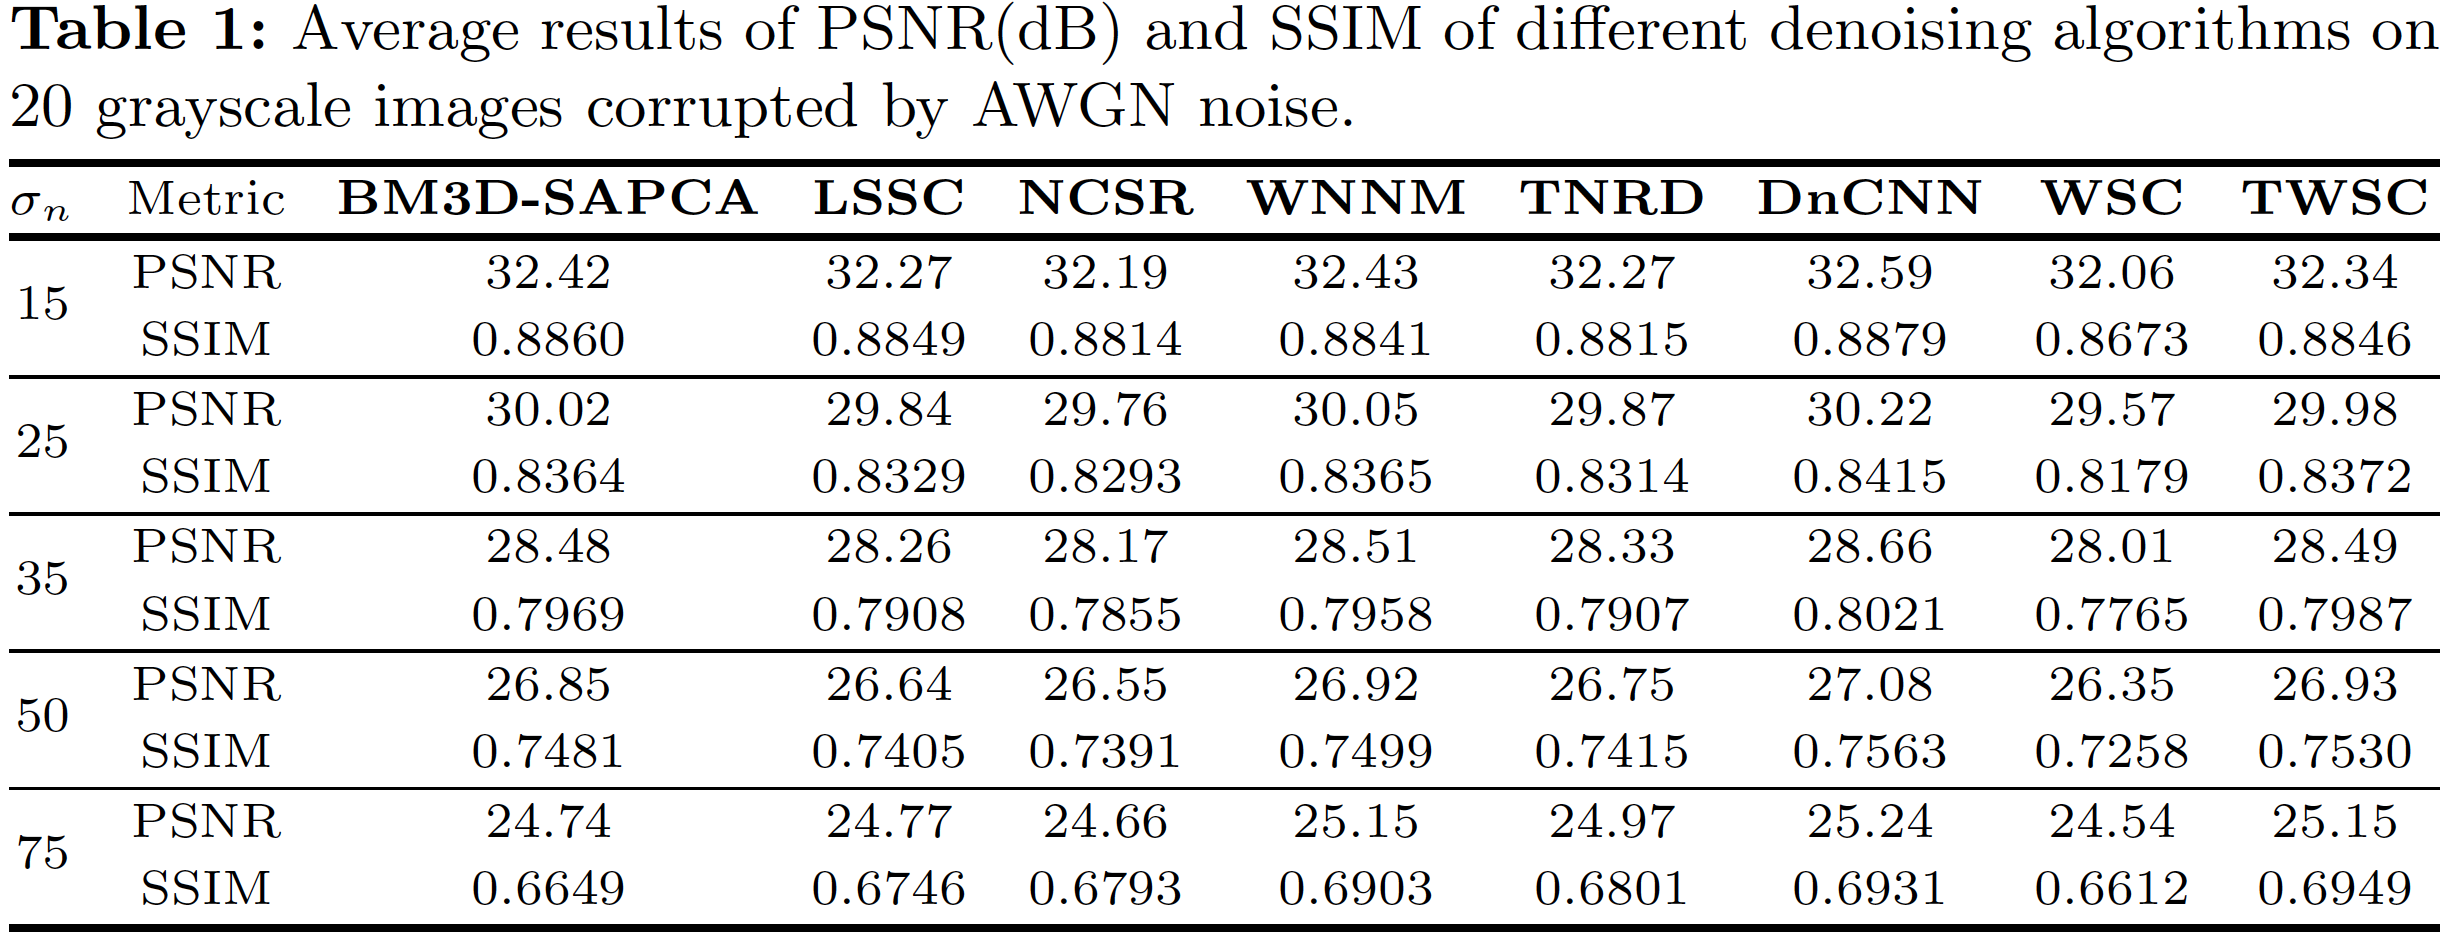
\includegraphics[width=\textwidth]{images/t1}
        \end{center}
    \end{minipage}
    \hfill
    \begin{minipage}[t]{0.49\textwidth}
    \textbf{\color{blue}Quantitative Comparisons on Realistic Noise Removal:}
        \begin{center}
            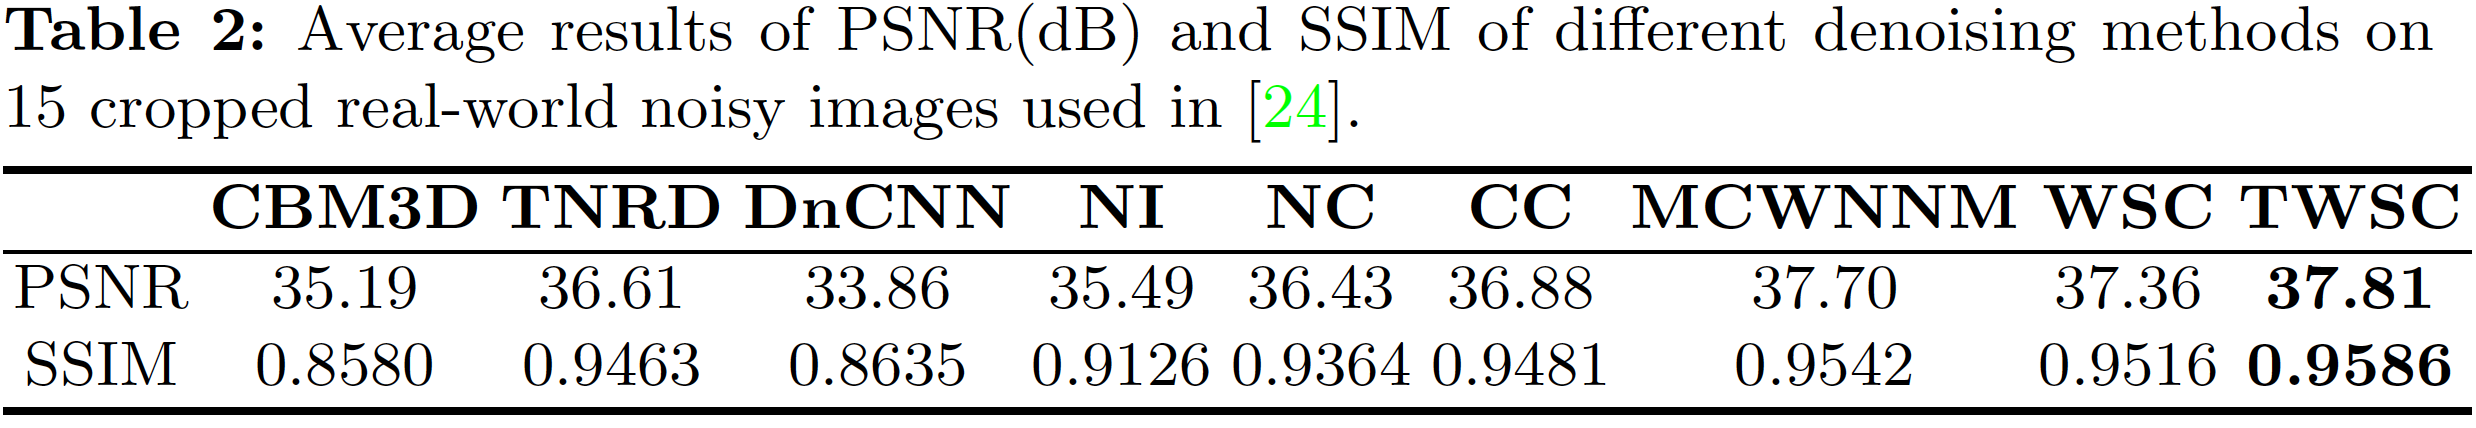
\includegraphics[width=\textwidth]{images/t2}
             \vspace{0mm}
          
            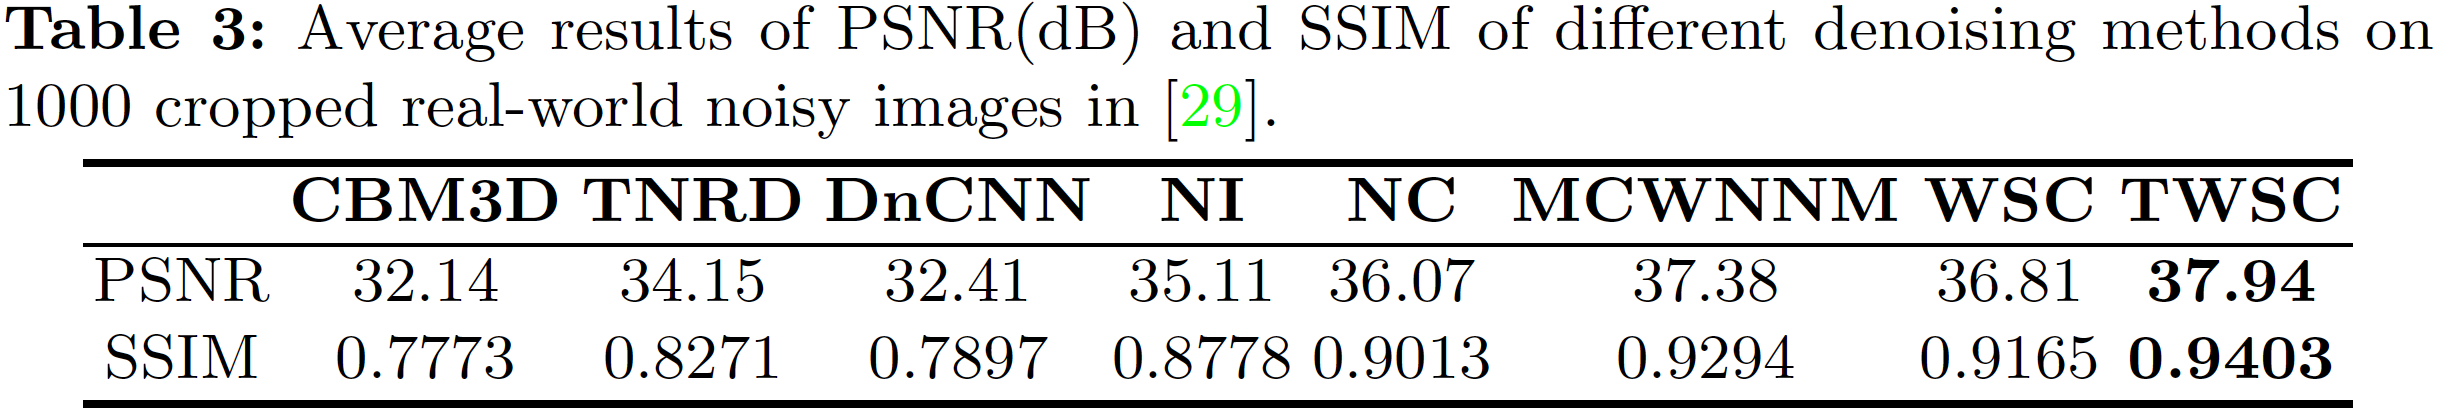
\includegraphics[width=\textwidth]{images/t3}
        \end{center}
    \end{minipage}

    \vspace{2mm}
    \begin{minipage}[t]{0.45\textwidth}
        \textbf{\color{blue}Comparisons on \textsl{Lena} (AWGN with $\sigma=75$):}
     \vspace{-2mm}
        \begin{center}
            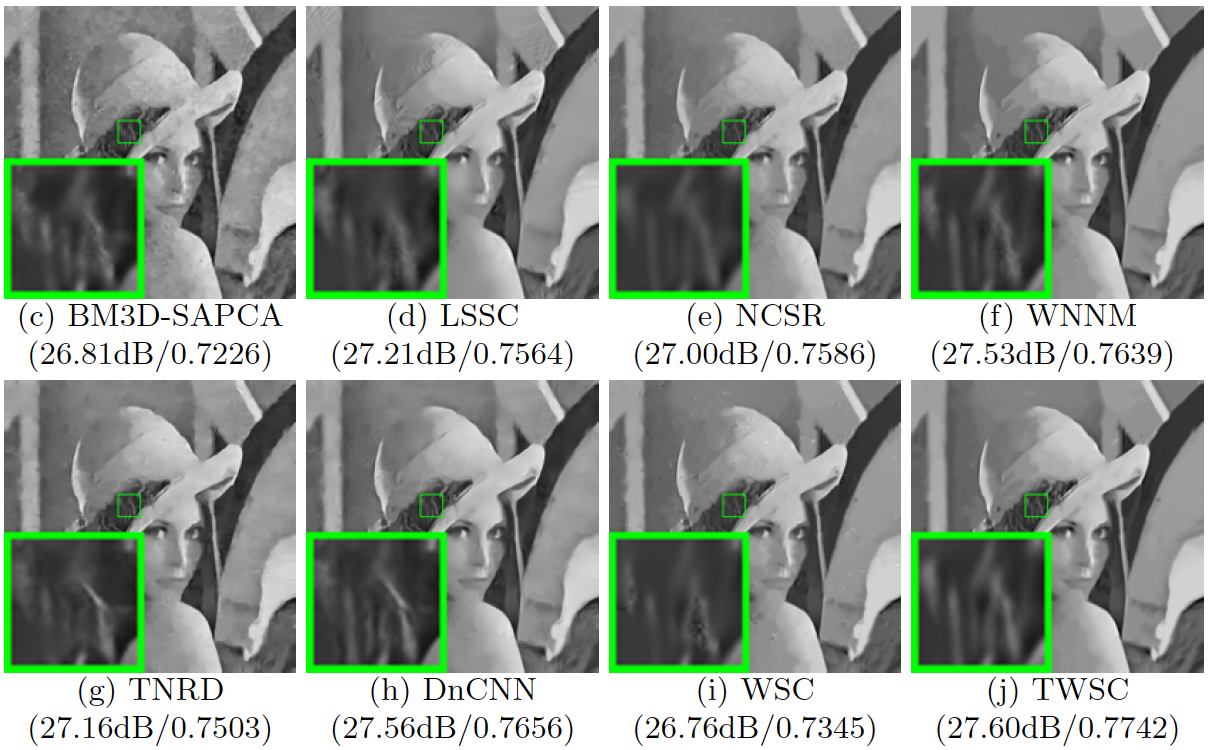
\includegraphics[width=\textwidth]{images/awgn}
        \end{center}
    \end{minipage}
    \hfill
    \begin{minipage}[t]{0.54\textwidth}
            \textbf{\color{blue}Comparisons on \textsl{Nikon D800 ISO 6400 1} in CC dataset [24]:}
        \vspace{-2mm}
        \begin{center}
            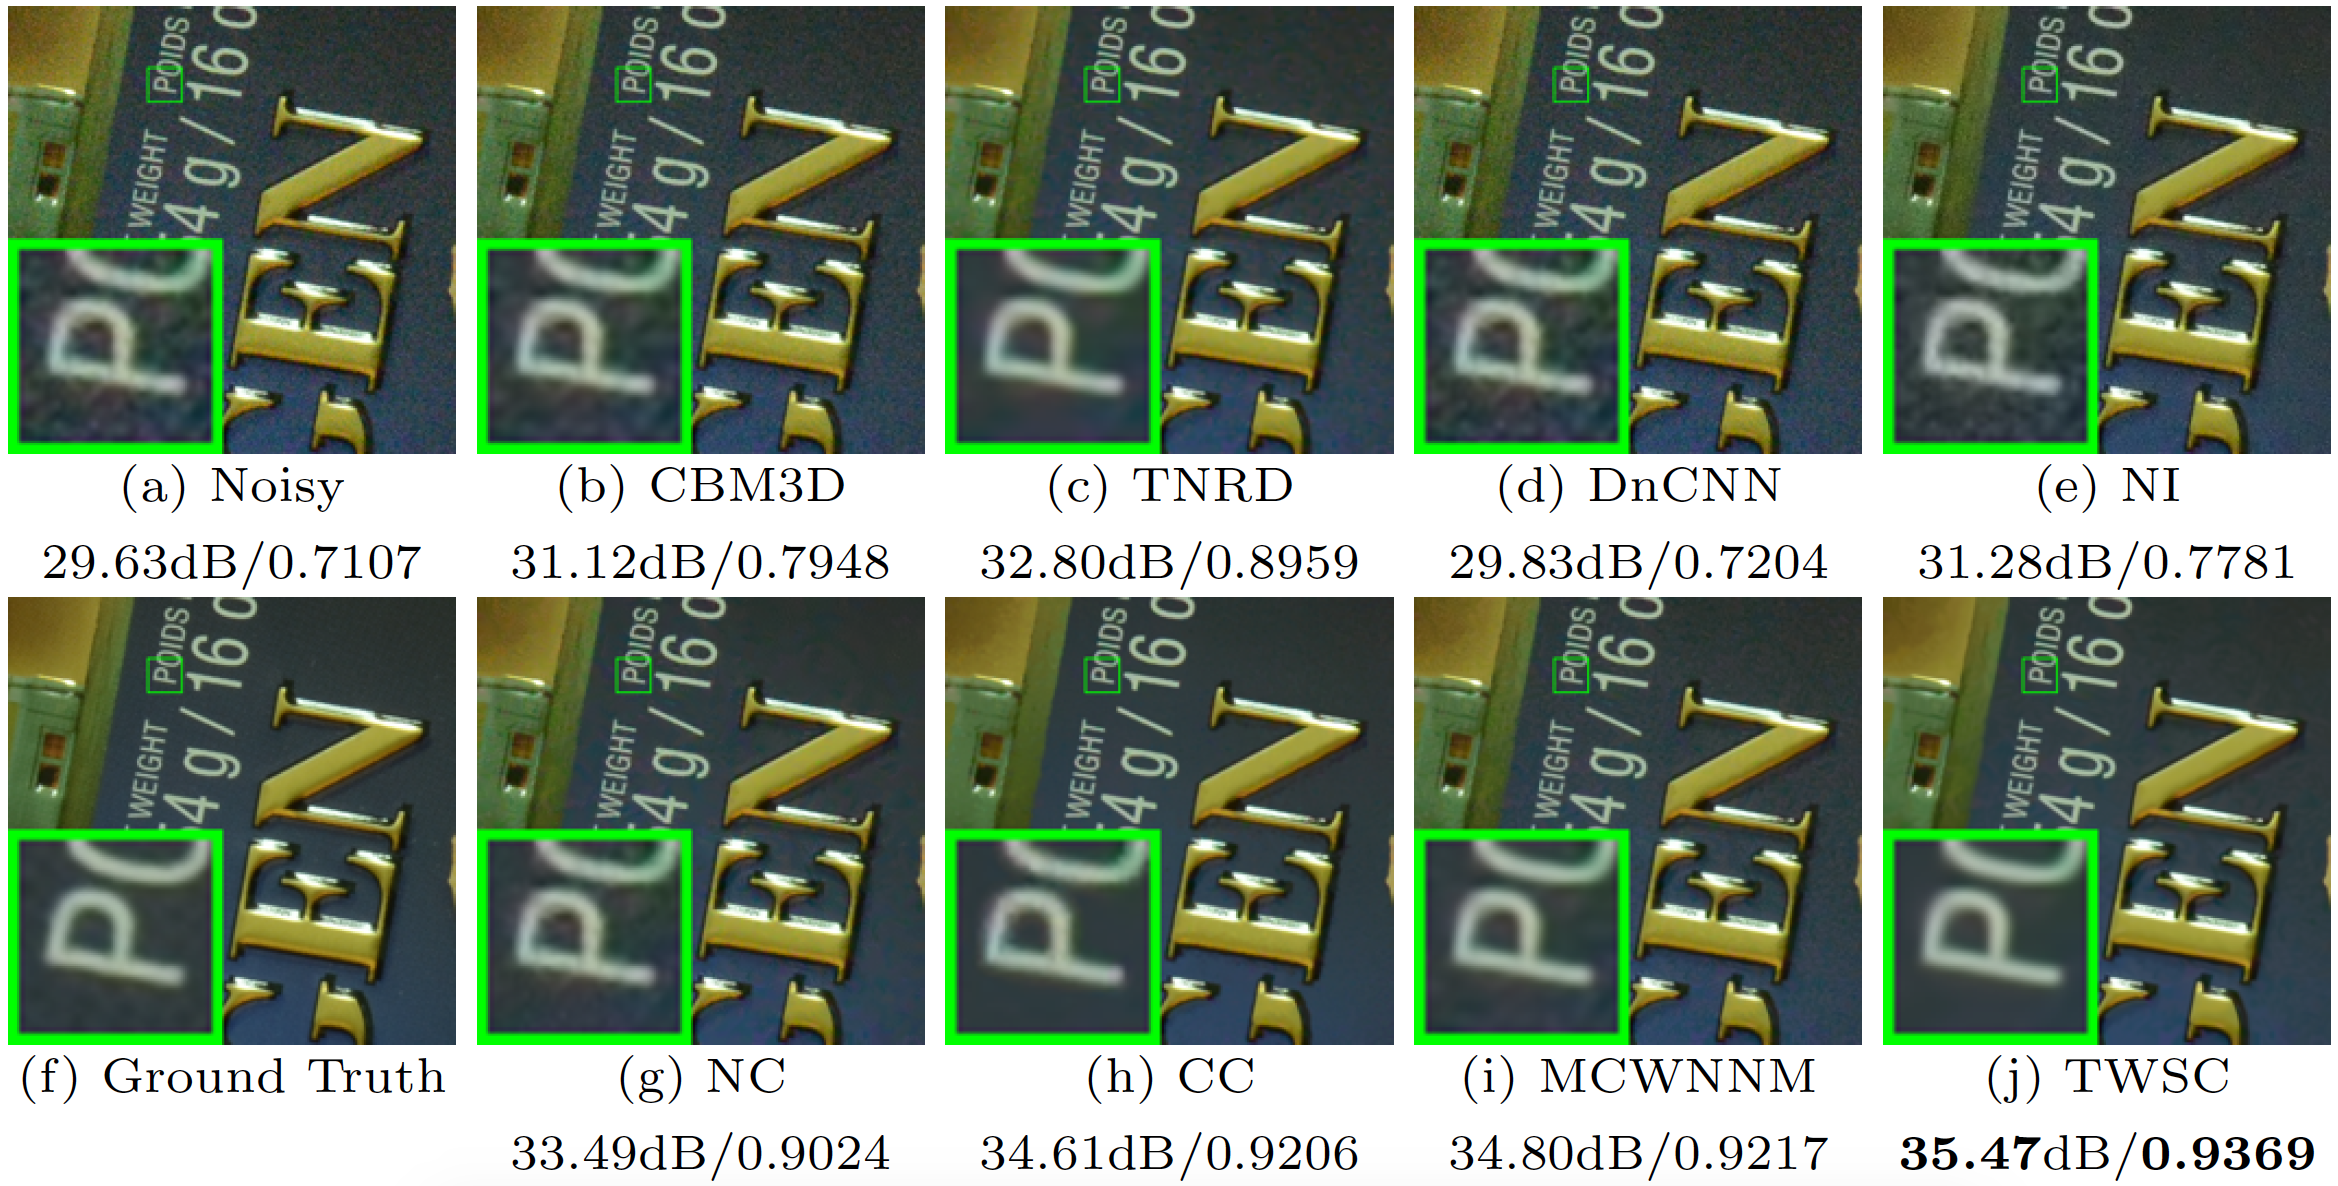
\includegraphics[width=\textwidth]{images/realcc}
        \end{center}
    \end{minipage}

\vspace{2mm}
    \begin{minipage}[t]{0.44\textwidth}
     \textbf{\color{blue}Quantitative Results on Speed:} 
        \vspace{-1mm}
        \begin{center}
            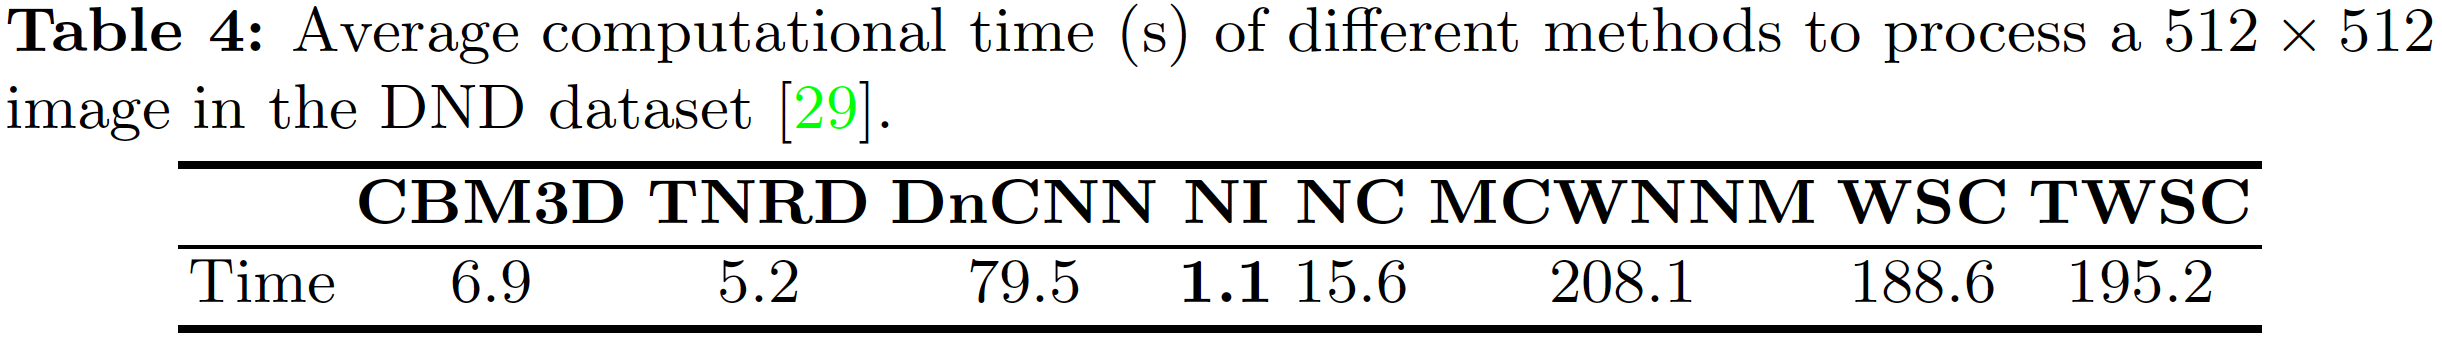
\includegraphics[width=\textwidth]{images/t4}
        \end{center}

        \begin{center}
        \begin{minipage}{0.55\linewidth}
            \begin{center}
            \textbf{Github Webpage}: \\
            \vspace{2mm}\textbf{Code} \& \textbf{Dataset}
            \end{center}
        \end{minipage}
        \begin{minipage}{0.4\linewidth}
            \begin{center}
                
\includegraphics[width=\linewidth]{images/TWSC_QRCode.png}
            \end{center}
        \end{minipage}
        \end{center}
    \end{minipage}
      \hfill
    \begin{minipage}[t]{0.55\textwidth}
            \textbf{\color{blue}Comparisons on \textsl{0001\_2} captured by Nexus 6P in DND dataset [29]:} 
        \vspace{-1mm}
        \begin{center}
            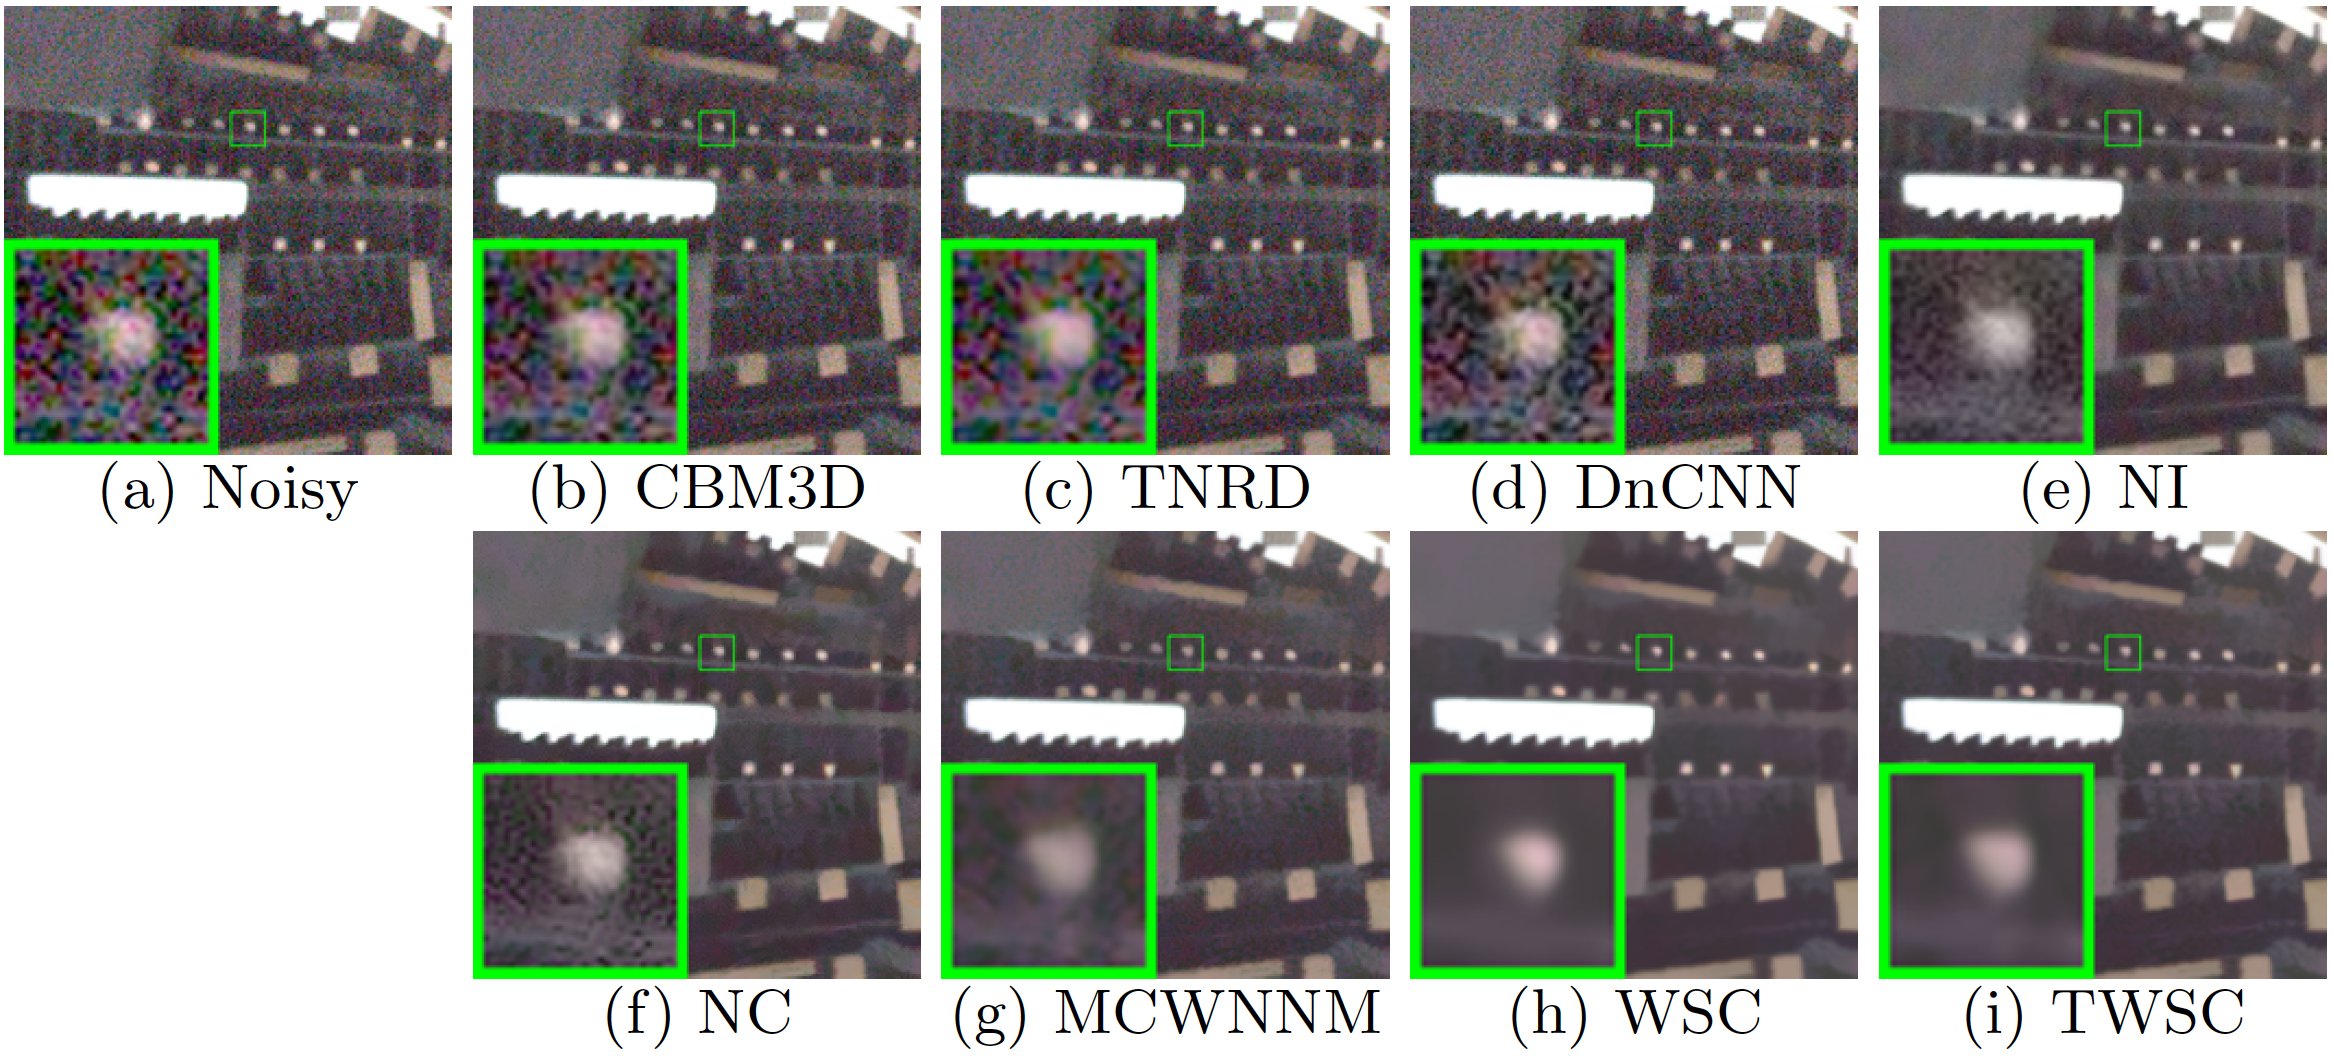
\includegraphics[width=\textwidth]{images/realdnd}
        \end{center}
    \end{minipage}
}

\headerbox{\bf\color{blue} The TWSC Scheme}{name=TWSC,column=0,below=contribution,span=2}{ 
\textbf{\color{blue}TWSC:} Given a color image patch $\mathbf{Y}=\mathbf{X}+\mathbf{N}\in{3p^2\times N}$ and $\mathbf{Y}=\mathbf{D}\mathbf{S}\mathbf{V}^{\top}$ is the SVD of $\mathbf{Y}$. The TWSC model can be written as
\vspace{-4mm}
\begin{equation}
\vspace{-4mm}
\label{e4}
\hat{\mathbf{C}}=\arg\min_{\mathbf{C}}\|\mathbf{W}_{1}(\mathbf{Y}-\mathbf{D}\mathbf{C})\mathbf{W}_{2}\|_{F}^{2}+\|\mathbf{W}_{3}^{-1}\mathbf{C}\|_{1}.
\end{equation}
The estimation of $\mathbf{X}$ can be $\hat{\mathbf{X}}=\mathbf{D}\hat{\mathbf{C}}$.

\textbf{\color{blue}Formulation of weight matrices:}
\vspace{-3mm}
\begin{equation}
\vspace{-3mm}
\begin{split}
\label{e9}
\mathbf{W}_{1}
&
=
\text{diag}(\sigma_{r}^{-1/2}\mathbf{I}_{p^2},\sigma_{g}^{-1/2}\mathbf{I}_{p^2},\sigma_{b}^{-1/2}\mathbf{I}_{p^2})
,
\\
\mathbf{W}_{2}
&
=
\text{diag}(\sigma_{1}^{-1/2},...,\sigma_{M}^{-1/2})
,
\mathbf{W}_{3} 
= 
\mathbf{S}
,
\end{split}
\end{equation}

\textbf{\color{blue}Visualization of weight matrices:}
        \begin{center}
        \vspace{-3mm}
        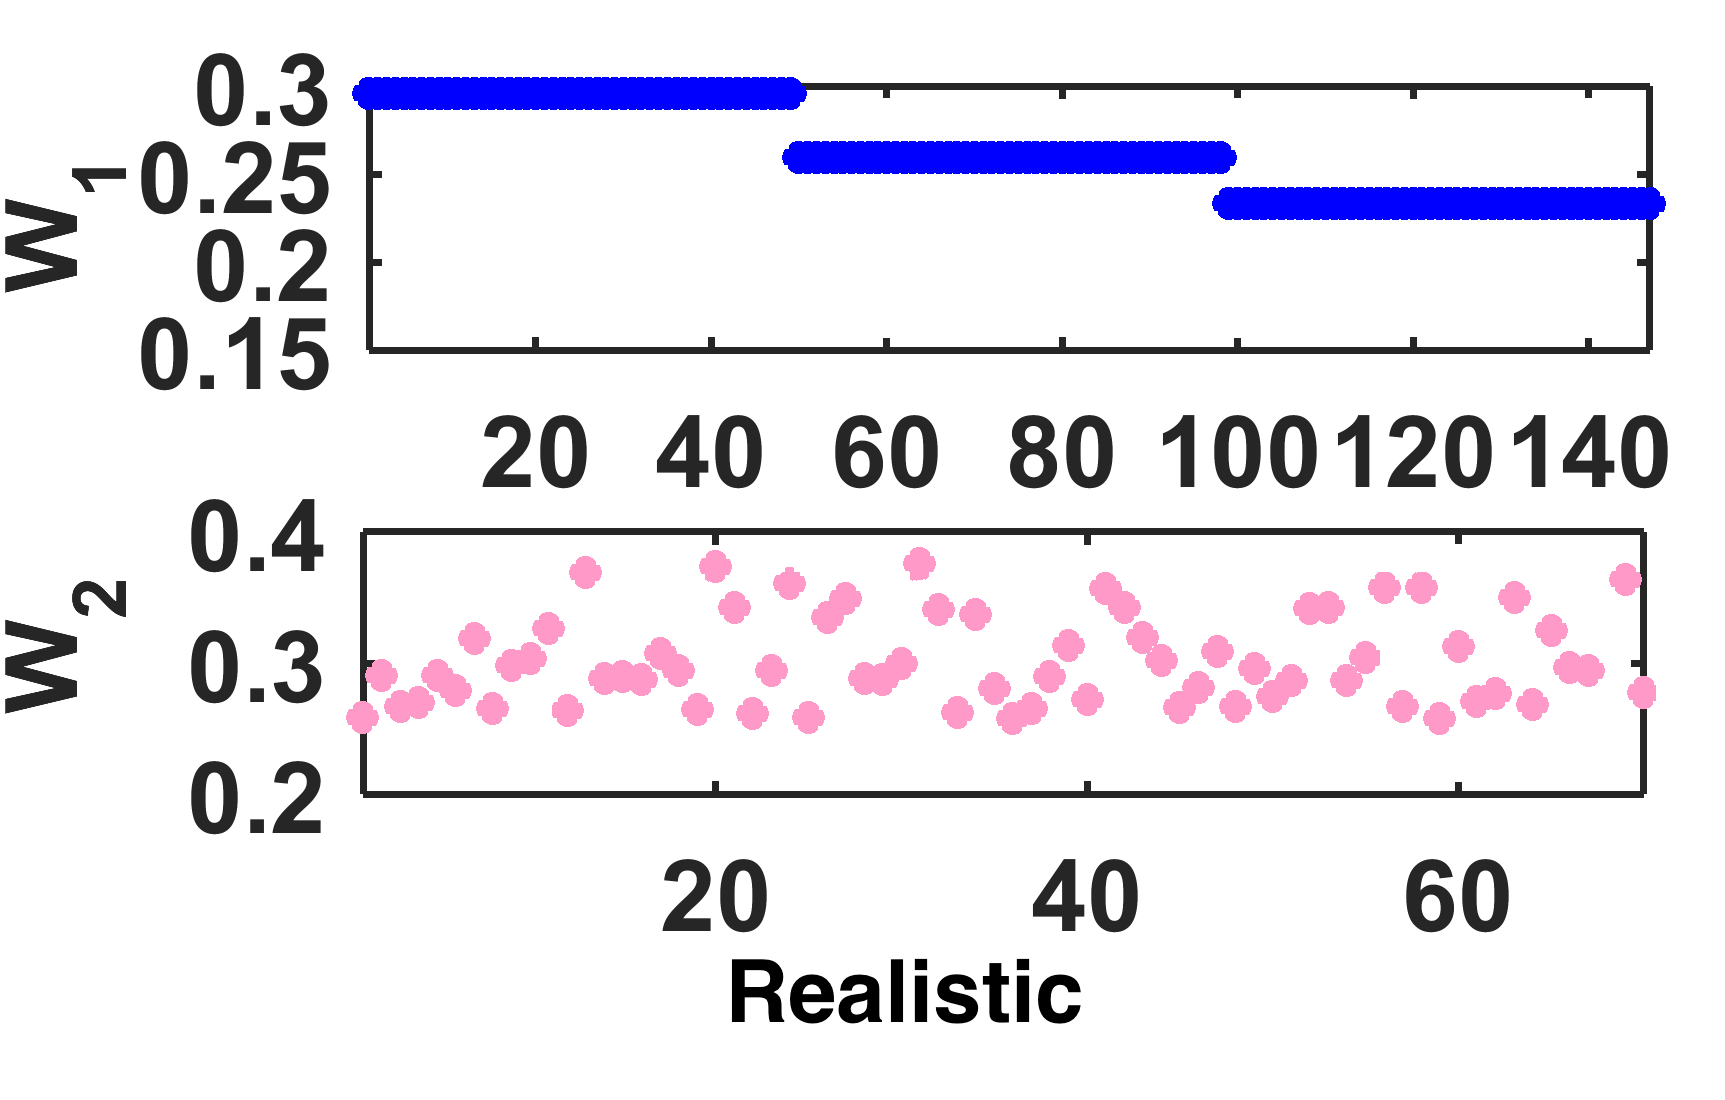
\includegraphics[width=0.48\linewidth]{images/wsreal2}
        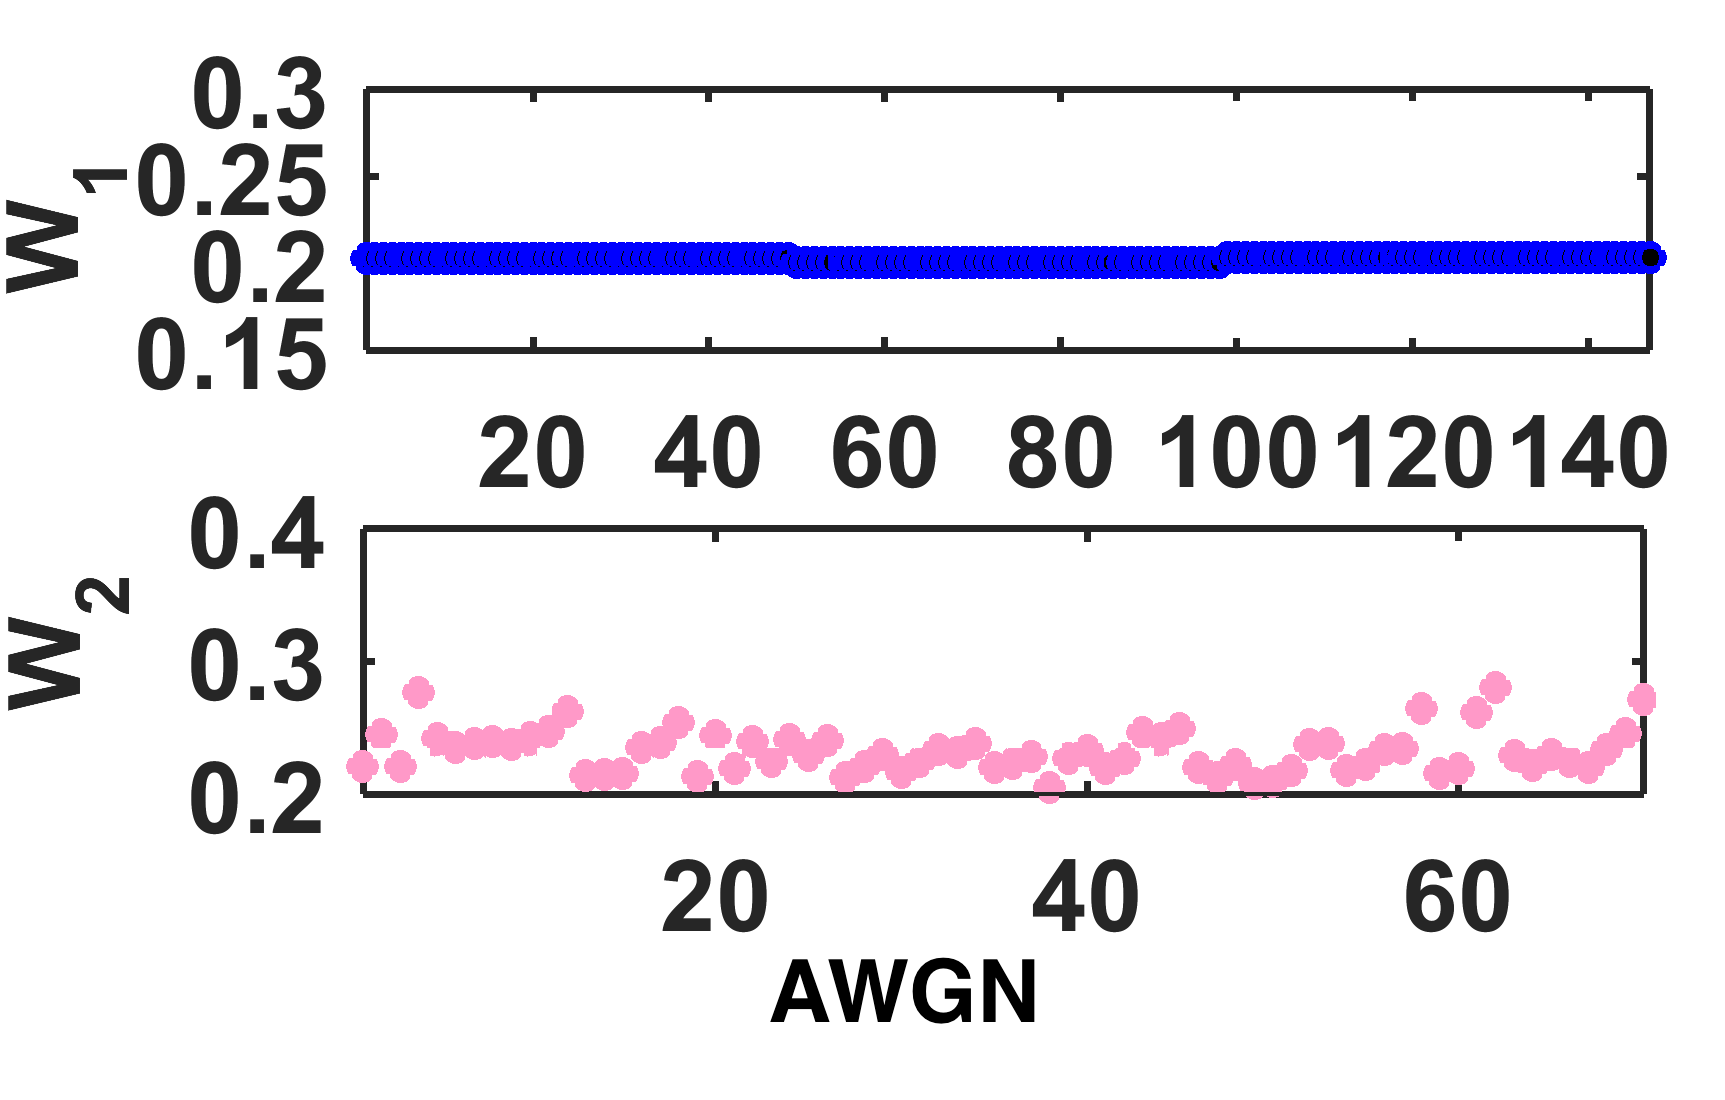
\includegraphics[width=0.48\linewidth]{images/wsgaussian2}
    \end{center}
    \vspace{-4mm}
}

%%%%%%%%%%%%%%%%%%%%%%%%%%%%%%%%%%%%%%%%%%%%%%%%%%%%%%%%%%%%%%%%%%%%%%%%%%%%%%
\headerbox{\bf\color{blue} Optimization}{name=optimization,column=0,below=TWSC,span=2}{
\textbf{\color{blue}Variable Splitting:} $\min_{\mathbf{C},\mathbf{Z}}\|\mathbf{W}_{1}(\mathbf{Y}-\mathbf{D}\mathbf{W}_{3}\mathbf{C})\mathbf{W}_{2}\|_{F}^{2}
+
\|\mathbf{Z}\|_{1}
\ 
\text{s.t.}
\ 
\mathbf{C}=\mathbf{Z}.
$

\textbf{\color{blue}ADMM:}
 
\quad\quad(a) $\mathbf{C}_{k+1}=\arg\min_{\mathbf{C}}\|\mathbf{W}_{1}(\mathbf{Y}-\mathbf{D}\mathbf{W}_{3}\mathbf{C})\mathbf{W}_{2}\|_{F}^{2}
+\frac{\rho_{k}}{2}\|\mathbf{C} - \mathbf{Z}_{k} + \rho_{k}^{-1}\mathbf{\Delta}_{k}\|_{F}^{2}.$

\quad\quad\quad\quad The solution $\mathbf{C}_{k+1}$ satisfies $\mathbf{A}\mathbf{C}_{k+1}+\mathbf{C}_{k+1}\mathbf{B}_{k}=\mathbf{E}_{k}$, where

\quad\quad\quad\quad$\mathbf{A}=\mathbf{W}_{3}^{\top}\mathbf{D}^{\top}\mathbf{W}_{1}^{\top}\mathbf{W}_{1}\mathbf{D}\mathbf{W}_{3}, \mathbf{B}_{k}=\frac{\rho_{k}}{2}(\mathbf{W}_{2}\mathbf{W}_{2}^{\top})^{-1}$,

\quad\quad\quad\quad$\mathbf{E}_{k}=\mathbf{W}_{3}^{\top}\mathbf{D}^{\top}\mathbf{W}_{1}^{\top}\mathbf{W}_{1}\mathbf{Y}+(\frac{\rho_{k}}{2}\mathbf{Z}_{k} -\frac{1}{2}\mathbf{\Delta}_{k})(\mathbf{W}_{2}\mathbf{W}_{2}^{\top})^{-1}$.

\quad\quad\quad\quad (\textcolor{red}{Solution}) $\mathbf{C}_{k+1}=\text{vec}^{-1}((\mathbf{I}_{M}\otimes\mathbf{A}+\mathbf{B}_{k}^{\top}\otimes\mathbf{I}_{3p^2})^{-1}\text{vec}(\mathbf{E}_{k}))$.

\quad\quad\quad\quad \textcolor{red}{Challenge: Is $(\mathbf{I}_{M}\otimes\mathbf{A}+\mathbf{B}_{k}^{\top}\otimes\mathbf{I}_{3p^2})^{-1}$ exist?}

\quad\quad(b) $\mathbf{Z}_{k+1}=\arg\min_{\mathbf{Z}}\frac{\rho_{k}}{2}\|\mathbf{Z} - (\mathbf{C}_{k+1}+\rho_{k}^{-1}\mathbf{\Delta}_{k})\|_{F}^{2}+\|\mathbf{Z}\|_{1}.$

\quad\quad(c) $\mathbf{\Delta}_{k+1}=\mathbf{\Delta}_{k} + \rho_{k}(\mathbf{C}_{k+1}-\mathbf{Z}_{k+1}).$

\quad\quad(d) $\rho_{k+1}= \mu\rho_{k}$, where $\mu\ge1$.

 }

\end{poster}
\end{document}
